\section{Limitations and Future Work}

In this section we discuss some limitations of our work and future research directions. The first limitation is the color map we use to depict the data in our cartograms. We use D3's built-in interpolateRdYlGn color map, a diverging color scheme of red, yellow, and green. However, we believe that the choice of color map can have a significant impact on the legibility of cartograms. In the user study, we carefully avoid extreme values where the location or color of the CCG makes it easier to locate the target. See \Cref{fig:extreme} for an example. We plan to explore the impact of different color maps on the legibility of cartograms in future work.

{
    \begin{figure}[tb!]
        \centering
        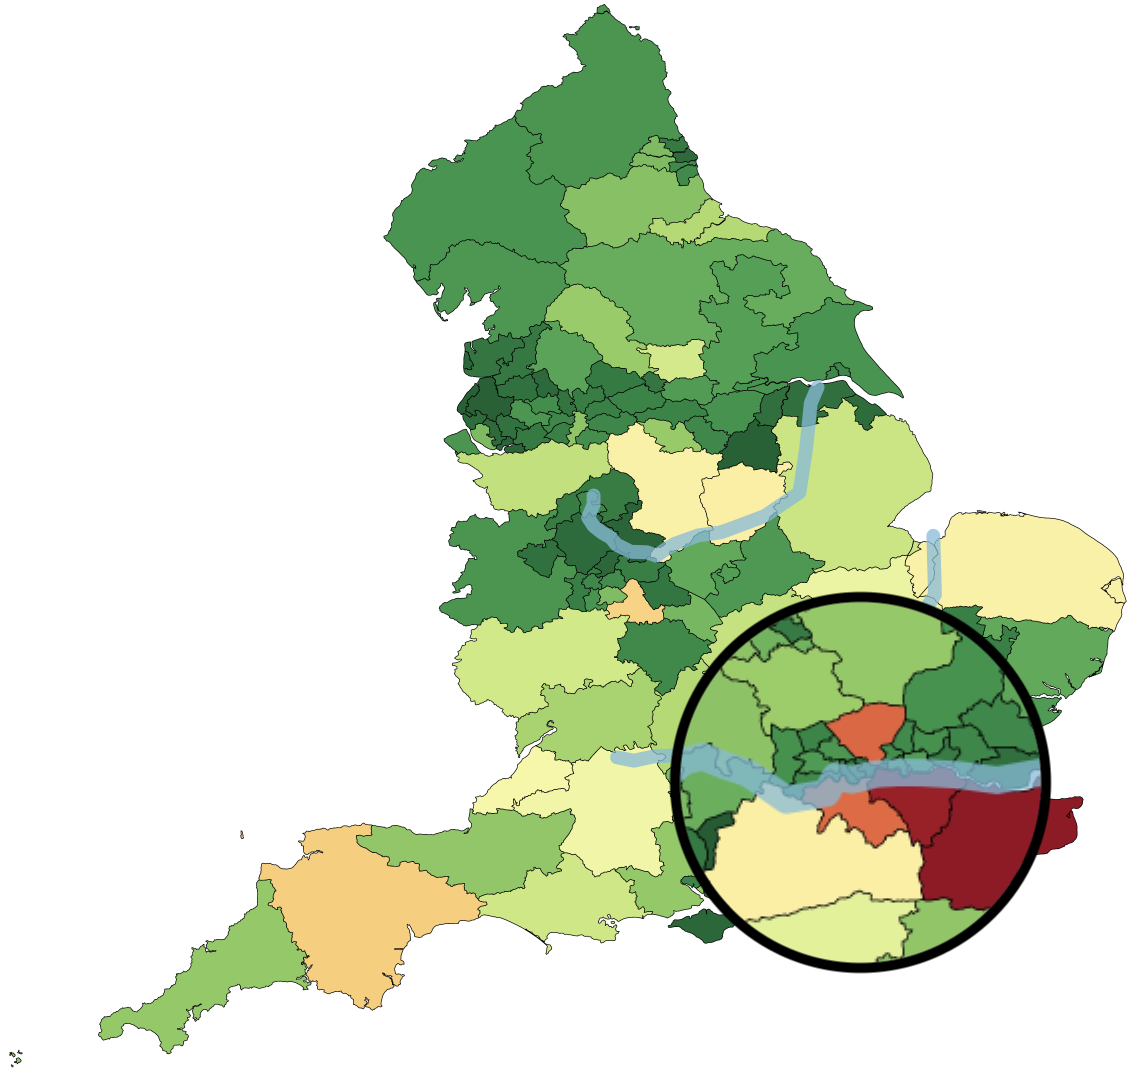
\includegraphics[width=\columnwidth,keepaspectratio]{figure/limitations/extreme.png}
        \caption{Due to color and relative location, we believe the CCGs in the black circle are easier to locate.}
        \label{fig:extreme}
    \end{figure}
}

Another limitation is the overlap removal algorithm (FNOR) we use. We believe that developing a new algorithm with built-in constraint support can significantly reduce the time needed to generate cartograms with rivers.
